\documentclass{article}
\usepackage{amsmath, tikz, tcolorbox, array, multicol, sfmath, enumerate, pgfplots}
\renewcommand{\familydefault}{\sfdefault}
\pgfplotsset{compat=newest}
\usetikzlibrary{arrows.meta}
\everymath{\displaystyle}
\tikzset{>=stealth}
\usepackage[top = 0.25in, bottom = 0.25in, left = 1.25in, right = 1.25in]{geometry}
\pagestyle{empty}
\raggedright

\newcounter{example}[section]
\newenvironment{example}[1][]{\refstepcounter{example}\par\medskip
   {\color{red}\textbf{Example~\theexample. #1}}}{\medskip}

\begin{document}

\section*{Derivatives}

\begin{tcolorbox}[colframe=orange!70!white, coltitle=black, title=\textbf{Summary}]
\begin{enumerate}
    \item The derivative $\left(\text{often denoted }y', \, f'(x), \, \text{ or } \frac{dy}{dx}\right)$ is a major component of calculus.
    \item The derivative of a function is the limit as $h$ approaches 0 of the difference quotient:
    \[f'(x) = \lim_{h \to 0} \frac{f(x+h)-f(x)}{h}\]
\end{enumerate}
\end{tcolorbox}
\vspace{1in}

\subsection*{Average Rate of Change and Limits}

Recall that the average rate of change of a function in an interval is the slope of the line connecting the points at those interval values:

\[
\frac{\Delta y}{\Delta x} = \frac{f(x_2)-f(x_1)}{x_2-x_1}
\]
\vspace{0.5in}

But what happens as the difference between $x_2$ and $x_1$ approaches 0? \newline\\

In other words, what is $\lim_{\Delta x \to 0}$ or what is $\lim_{x_2 \to x_1}$?
\vspace{1in}

\begin{example}
Find the average rate of change over each interval for the function $f(x) = x^2 + 1$.
\begin{multicols}{3}
\begin{enumerate}[(a)]
    \item $[3, 3.001]$
    \item $[3, 3.0001]$
    \item $[3, 3.00001]$
\end{enumerate}
\end{multicols}
\vfill 
\begin{enumerate}[(a)]  \setcounter{enumi}{3}
    \item What is $\lim_{\Delta x \to 0}$?
\end{enumerate}
\end{example}
\vspace{0.75in}

\newpage 

The answer in Example 1d is the {\color{orange}\textbf{derivative}} of $f(x) = x^2 + 1$ at the point $x = 3$.
\vspace{0.5in}

\textbf{It will tell us the slope of the line tangent to the curve at $\pmb{x = 3}$.} \newline\\

\begin{center}
    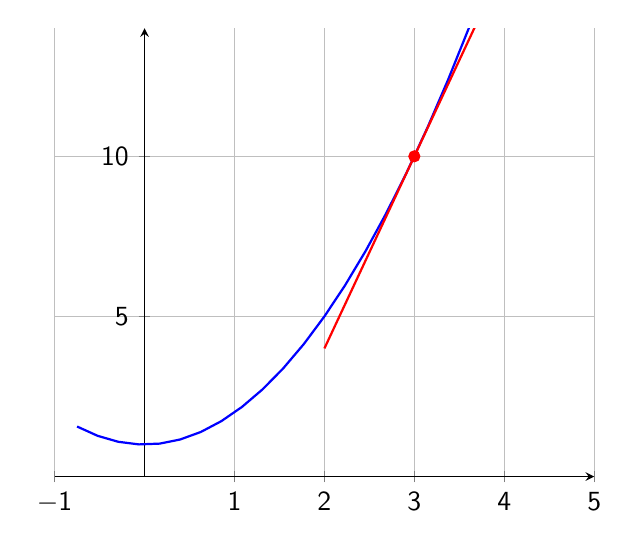
\begin{tikzpicture}
    \begin{axis}
    [axis lines = middle, xmin = -1, xmax = 5, ymin = 0, ymax = 14, grid]
    \addplot [blue, thick, domain=-0.75:4.75] {x*x + 1};
    \addplot [mark = *, red] coordinates {(3,10)};
    \addplot [red, domain=2:4, thick] {6*x-8};
    \end{axis}
    \end{tikzpicture}
\end{center}
\vspace{0.5in}

But what if we want to find the derivative of a function not just at one value of $x$, but for \underline{all} values of $x$ in the function's domain?
\vspace{1in}

\subsection*{Interpreting Derivatives as a Limit of the Difference Quotient}

What is the slope of the line connecting the 2 points below? \newline\\

\begin{tikzpicture}
\begin{axis}
[axis lines = middle, xmin = -2, xmax = 5, ymin = -2, ymax = 6,
xtick={1,4}, xticklabels = {$x$, $x+h$}, ymajorticks=false, clip=false]
\addplot[<->, very thick, blue, smooth, domain=-2:5] plot {0.15*x^2 + 1};
\addplot[mark = *, only marks] coordinates {(1,1.15) (4,3.4)};
\node at (axis cs: 1,1.15) [below] {$(x, f(x))$};
\node at (axis cs: 4.1,3.4) [right] {$(x+h, f(x+h))$};
\end{axis}
\end{tikzpicture}
\vfill 

\newpage 

The {\color{violet}\textbf{difference quotient}} of a function is defined as
\[ \frac{f(x+h)-f(x)}{h} \]
\vspace{1in}

This is a 3-step process:
\begin{enumerate}
    \item Evaluate $f(x+h)$; a function composition
    \item Subtract the given function, $f(x)$
    \item Divide previous result by $h$ and simplify
\end{enumerate}

\vspace{1.25in}

% \newpage 

\begin{example}
Find the difference quotient of each.
\begin{enumerate}[(a)]
    \item $f(x) = x^2$  \vfill 
    \item $f(x) = 5x^2$ \vfill \newpage  
    \item $f(x) = x^2 - 2x$ \vfill 
    \item $f(x) = 7$ \vfill 
\end{enumerate}
\end{example}

The {\color{blue}\textbf{derivative}} is the limit of the difference quotient as $h$ approaches 0.    \newline\\

\[
\boxed{\boxed{
f'(x) = \lim_{h\to 0} \frac{f(x+h)-f(x)}{h}
}}
\]
\vspace{0.5in}

% \textsc{Other Derivative Notations}:  \[\frac{dy}{dx} \qquad y' \qquad \dot{x}\]
\newpage

\begin{example} \label{deriv}
Find the derivative of each.
\begin{enumerate}[(a)]
    \item $f(x) = x$ \vfill 
    \item $f(x) = x^2$ \vfill   \newpage 
    \item $f(x) = 5x^2$        \vfill 
    \item $f(x) = x^2-2x$       \vfill \newpage 
    % \item $f(x) = x^3 - 5$ \quad \emph{Hint:} $(x+h)^3 = x^3 + 3x^2h + 3xh^2 + h^3$     \vfill 
    \item $f(x) = 7$    \vspace{2.5in} 
\end{enumerate}
\end{example}

\textsc{Other Common Notations for Derivatives}: $\frac{dy}{dx}$ and $y'$
\vspace{1in}

When you evaluate a derivative at an $x$-value, you are finding the slope of the line tangent to the curve there. \newline\\

This is also called finding the \emph{instantaneous rate of change}.
\vfill 

\begin{example}
Find each of the following. 
\begin{multicols}{2}
\begin{enumerate}[(a)]
    \item $f'(5)$ from Example \ref{deriv}(a).
    \item $f'(0)$ from Example \ref{deriv}(b).
\end{enumerate}
\end{multicols}
\vfill 
\begin{enumerate}[(a)] \setcounter{enumi}{2}
    \item $f'(-9)$ from Example \ref{deriv}(c).
\end{enumerate}
\end{example}
\vfill 

% Derivatives have may aliases:     
% \begin{itemize}
%         \item Instantaneous rate of change.
%         \item Tangent slope to a curve.
%         \item Limit as secant line becomes tangent line.    
% \end{itemize}
% \vspace{0.5in}

% In calculus, you will learn shortcuts so you won't always have to do what we did in these notes to find the derivative.


\end{document}
